% Please use the skeleton file you have received in the
% invitation-to-submit email, where your data are already
% filled in. Otherwise please make sure you insert your
% data according to the instructions in PoSauthmanual.pdf
\documentclass{PoS}
\usepackage{lipsum}

%\usepackage{subfigure}
%\usepackage{hepnames}
%\usepackage{hyperref}

%\usepackage[amssymb]{SIunits} %FIXME SIunits or siunitx ?
\usepackage[load-configurations=abbreviations,tight-spacing=true,separate-uncertainty,bracket-numbers = false]{siunitx} 

\usepackage{graphicx}% Include figure files
\usepackage{subfigure}
\usepackage{url}


\usepackage{lineno}
\setpagewiselinenumbers
\modulolinenumbers[5]

\usepackage{epstopdf}
\epstopdfsetup{
    suffix=,
}

%FIXME always copy this list to next telescope paper!
%general stuff 
\newcommand{\e}{\ensuremath{\mathnormal{e}}}
\newcommand{\h}{\ensuremath{\mathnormal{h}}}
\newcommand{\eV}{\ensuremath{\textrm{eV}}}
\newcommand{\cspeed}{\ensuremath{\mathnormal{c}}}
\newcommand{\dd}{\mathrm d}

%tscope specific
\newcommand{\DESY}{\ensuremath{\textrm{DESY}}}
\newcommand{\Datura}{\ensuremath{\textrm{DATURA}}}
\newcommand{\Duranta}{\ensuremath{\textrm{DURANTA}}}
\newcommand{\Mimosa}{\ensuremath{\textrm{MIMOSA\,26}}}
\newcommand{\noise}{\ensuremath{\xi_{\textrm{n}}}}
\newcommand{\epsdut}{\ensuremath{\mathnormal{\varepsilon_{\textrm{DUT}}}}}
\newcommand{\epssut}{\ensuremath{\mathnormal{\varepsilon_{\textrm{SUT}}}}}
\newcommand{\epsmimo}{\ensuremath{\mathnormal{\varepsilon_{\textrm{M26}}}}}
\newcommand{\dz}{\ensuremath{\textrm{d}z}}
\newcommand{\dzsut}{\ensuremath{\textrm{d}z_{\textrm{SUT}}}}
\newcommand{\xzero}{\ensuremath{\mathnormal{X}_0}}

%resolutions
\newcommand{\sigmap}{\ensuremath{\sigma_{\textrm{pointing}}}}
\newcommand{\sigmatu}{\ensuremath{\sigma_{\textrm{t,u}}}}
\newcommand{\sigmatb}{\ensuremath{\sigma_{\textrm{t,b}}}}
\newcommand{\sigmat}{\ensuremath{\sigma_{\textrm{t}}}}
\newcommand{\sigmapGBL}{\ensuremath{\sigma_{\textrm{p,GBL}}}}
\newcommand{\sigmameas}{\ensuremath{\sigma_{\textrm{meas}}}}
\newcommand{\sigmadut}{\ensuremath{\sigma_{\textrm{DUT}}}}
\newcommand{\sigmai}{\ensuremath{\sigma_{\textrm{int}}}}
\newcommand{\sigmam}{\ensuremath{\sigma_{\textrm{M26}}}}
\newcommand{\sigmahat}{\ensuremath{\hat{\sigma}_{\textrm{int}}}}
\newcommand{\sigmaslope}{\ensuremath{\sigma_{\textrm{slope}}}}
\newcommand{\sigmaeps}{\ensuremath{\sigma_{\textrm{eps}}}}
\newcommand{\sigmaedge}{\ensuremath{\sigma_{\textrm{edge}}}}

%positions
\newcommand{\zdut}{\ensuremath{z_{\textrm{DUT}}}}
\newcommand{\zzz}{\ensuremath{z_{3}}}

%residuals
\newcommand{\rbiased}{\ensuremath{r_{\textrm{b}}}}
\newcommand{\runbiased}{\ensuremath{r_{\textrm{u}}}}
\newcommand{\rhat}{\ensuremath{\hat{r}_{\textrm{b}}}}
\newcommand{\pb}{\ensuremath{p_{\textrm{b}}}}

%angles
\newcommand{\aeff}{\ensuremath{\alpha_{\textrm{eff}}}}

%software
\newcommand{\eudet}{\ensuremath{\textrm{EUDET}}}
\newcommand{\eudaq}{\ensuremath{\textrm{EUDAQ}}}
\newcommand{\EUTelescope}{\ensuremath{\textrm{EUTelescope}}}
\newcommand{\Geant}{\ensuremath{\textrm{Geant4}}}

%estimators
\newcommand{\rmshundred}{\ensuremath{\textrm{rms}_\textrm{100}}}
\newcommand{\rmsninety}{\ensuremath{\textrm{rms}_\textrm{90}}}
\newcommand{\gausshundred}{\ensuremath{\sigma_\textrm{100}}}
\newcommand{\gaussninety}{\ensuremath{\sigma_\textrm{95}}}
\newcommand{\studhundred}{\ensuremath{\textrm{t}_\textrm{100}}}
\newcommand{\studninety}{\ensuremath{\textrm{t}_\textrm{90}}}
\newcommand{\aadhundred}{\ensuremath{\textrm{AAD}_\textrm{100}}}
\newcommand{\aadninety}{\ensuremath{\textrm{AAD}_\textrm{90}}}

\title{Simulation of material budget measurements with beam telescopes}

\ShortTitle{Material budget measurements with beam telescopes}

\author{\speaker{Hendrik Jansen}\\
        DESY\\
        E-mail: \email{hendrik.jansen@desy.de}}

\author{Paul Sch\"utze\\
        DESY\\
        E-mail: \email{paul.schuetze@desy.de}}

\abstract{
High-precision particle tracking devices allow for a two-dimensional analysis of the material budget distribution of, e.g., particle detectors and their periphery.
These tracking devices, called beam telescopes, enable a precise measurement of the trajectory of charged particles with a position resolution of a few micrometer
and an angular resolution of the order of a few ten microradian.
In this contribution, the material budget of a structured aluminum cube is reconstructed from various estimators based on the deflection angles of simulated electron trajectories.
Electrons in the GeV-range serve as beam particles carrying enough momentum to traverse few millimetre thick targets
 whilst undergoing multiple Coulomb scattering in the target allowing for precise measurement of the deflection. 
Probing a target under various rotation angles %with respect to the beam axis
 enables a tomographic reconstruction of the target. 
 
We discuss the performance of width estimators of the scattering angle distributions and their impact on the contrast and the resolution of the reconstructed image. 
}

\FullConference{The 26th International Workshop on Vertex Detectors\\
		10-15 September, 2017\\
		Las Caldas, Asturias, Spain}


\begin{document}
\linenumbers
\section{Introduction}
%\lipsum
Charged particles undergo multiple Coulomb scattering while traversing material. 
The distribution of the angle between the incoming and the outgoing trajectory, i.e.\ before and after the material, is characterised by the amount of material budget traversed. 
The measurement of the width of such distributions offers to quantify the amount of material budget seen by the particle. 
Moli\`ere~\cite{moliere} postulated a theory without empirical parameters to describe multiple scattering in arbitrary materials.
Later, Gaussian approximations to the involved calculations of his theory have been developed e.g.\ by Highland~\cite{ref:scatteringhighland} in order to simplify predictions.

%Today, precise tracking detectors allow for the characterisation of unknown materials based on their scattering properties. %try to avoid single phrase paragraphs, I guess.
For this contribution, simulations have been performed replicating a 5\,GeV electron beam traversing a $\eudet$-type beam telescope \cite{JansenEPJ} and a structured aluminium cube serving as a sample under test. 
A track reconstruction is performed, enabling the extraction of the particle scattering angles at the target arising from the multiple scattering therein.
Various estimators are constructed in order to measure the width of the angular distribution, preferably  in a precise, robust and unbiased manner. 
As the angular distribution may vary largely from a normal distribution and presents with noticeable tails,
 we evaluate the impact of the choice of the estimator on the reconstructed image in terms of contrast and resolution. 


\section{Simulation set-up}
% Describe setup, sensors and sample
For the simulation presented, the AllPix~\cite{ref:AllPix} detector simulation framework was used, which is based on $\Geant$ libraries~\cite{Agostinelli2003250,1610988}.
The libraries feature realistic models of the interaction of a high-energy particle beam with matter including multiple Coulomb scattering processes.
Furthermore, the AllPix framework allows for the definition of active sensor volumes, emulating the response of particle detectors using a data-driven digitization process. 

\begin{figure}[!bp]
	\center
	\includegraphics[trim= 50 180 220 20, width=.55\linewidth]{figures/sketch_tscope.eps}
	\hspace{30pt}
	\raisebox{40pt}{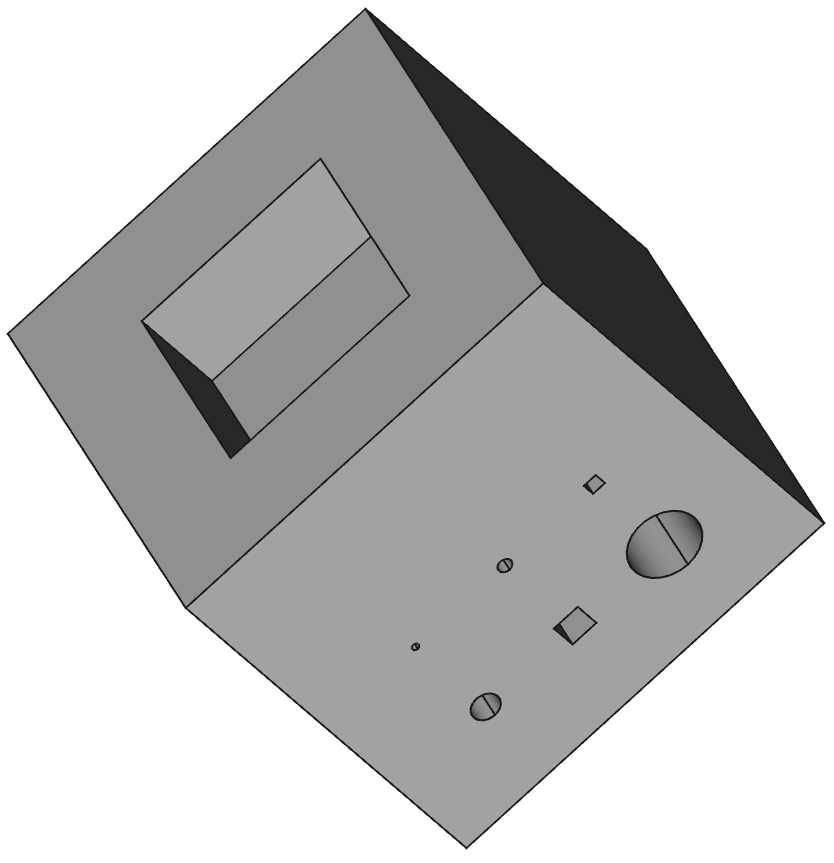
\includegraphics[trim= 0 0 0 0, width=.21\linewidth]{figures/phantomTest.png}}
	\caption[Sketch of the Datura beam telescope]{%
	Sketch of the $\Datura$ beam telescope (left) with its six pixel detector planes and the sample under test (SUT) shown in 3D (right). % with six sensor planes and a sample under test in the centre (left). 
	The sample, shown in 3D (right), consists of a $\SI{6}{m\meter}$ aluminium cube with a rectangular cut-out as well as round and rectangular holes of different sizes.
	}
	\label{fig:setup}
\end{figure}

The simulation mimics a realistic set-up, as it can be realised at the DESY Test Beam Facility~\cite{ref:DESYtb}. 
Six pixelated  silicon sensor planes, representing the DATURA beam telescope~\cite{JansenEPJ}, are positioned around a sample under test (SUT), cf.\ Fig.~\ref{fig:setup}~(left). 
%The sensor planes resemble six MIMOSA 26 fine-pitch pixel sensors. 
%With a pixel pitch of $\SI{18.4}{\mu}\times \SI{18.4}{\mu}$ and an array of 1152 columns and 576 rows, each sensor covers a total area of $\SI{21.2}{m\meter}\times\SI{10.6}{m\meter}$. 
For every simulated particle traversing the pixel sensor planes, a sensor response is calculated. 
The simulated response consists of clusters of one or more registered pixels,
 depending on the impact position of the particle, and is trimmed to its measured response~\cite{ref:datura-inpixel}.
% The intrinsic sensor resolution has been measured to be $\SI{3.24}{\mu}$.

The simulated SUT, shown in Fig.~\ref{fig:setup} (right), is an aluminium cube with an edge length of $\SI{6}{\mm}$,
 featuring a rectangular cut-out of $\SI{3}{\mm}\times\SI{3}{\mm}\times\SI{1.5}{\mm}$ at the bottom side. 
Furthermore, squared and round holes ranging from $\SI{0.1}{\mm}$ to $\SI{1}{\mm}$ in size and diameter are added.% in order to investigate on the visibility of small structures.

In the chosen configuration of the beam telescope,
 the sample is placed in the centre of the beam telescope, half way between plane\,2 and plane\,3, as shown in Fig.~\ref{fig:setup}. %counting (``second'' is ambigious ...)
The distance $\dzsut$ between the SUT and the neighbouring sensors is to be minimised for optimal pointing resolution at the sample,
 whereas the distance $\dz$ between two sensor planes is maximised for improved angular resolution.
Here, the distances were chosen to be $\dzsut =\SI{10}{\mm}$ and $\dz=\SI{150}{\mm}$, again representing a realistic choice. 

An electron beam with a mean momentum of 5\,GeV/$\cspeed$, a Gaussian momentum spread of 0.15\,GeV/$\cspeed$, and a divergence of $\SI{1}{\milli\radian}$ is used to fully illuminate the sample. 

The $\Geant$ libraries include physics models emulating, among other things, energy losses due to ionisation and scattering processes.
Charged particles traversing any material are deflected by the electric field of the nuclei, resulting in an effective deflection of the particle in the transverse plane when leaving the material,
 which depends on the traversed material budget $\varepsilon_{\textrm{SUT}} = d / \xzero$ of the sample. 
The parameter $\xzero$ denotes the radiation length of the material and is tabulated in reference~\cite{ref:pdg2016}. 
As an approximation to the Moliere theory, the distribution of scattering angles follows a normal distribution with the variance given by~\cite{ref:scatteringhighland, ref:pdg2016} 

\begin{equation}
 \Theta_0^2 = \left( \frac{\SI{13.6}{\mega\eV}}{\beta \cspeed p}\cdot z \right)^2 \cdot \varepsilon \cdot \big( 1+0.038\cdot\ln(\varepsilon) \big)^2\,,
 \label{eq:highland}
\end{equation}

\noindent
with the particle's velocity $\beta \cspeed$, its momentum $p$ and its charge number $z$ and the material budget $\varepsilon$. 
Hence the material budget and therefore the material properties of a sample can be extracted from a measurement of the scattering angle distribution.

%In order to account for an inhomogeneous response of the measurement system,
% the measurement of such distributions for homogeneous samples of known material type and thickness can be used to calibrate the measured response, as implied in~\cite{ref:X0}.

\section{Material budget estimators}

\begin{figure}[t!]
  \centering
  %\includegraphics[width=0.49\textwidth]{img/run28_1GeV_01mm_gblsumkxandsumky_xyP_mean.eps}  
  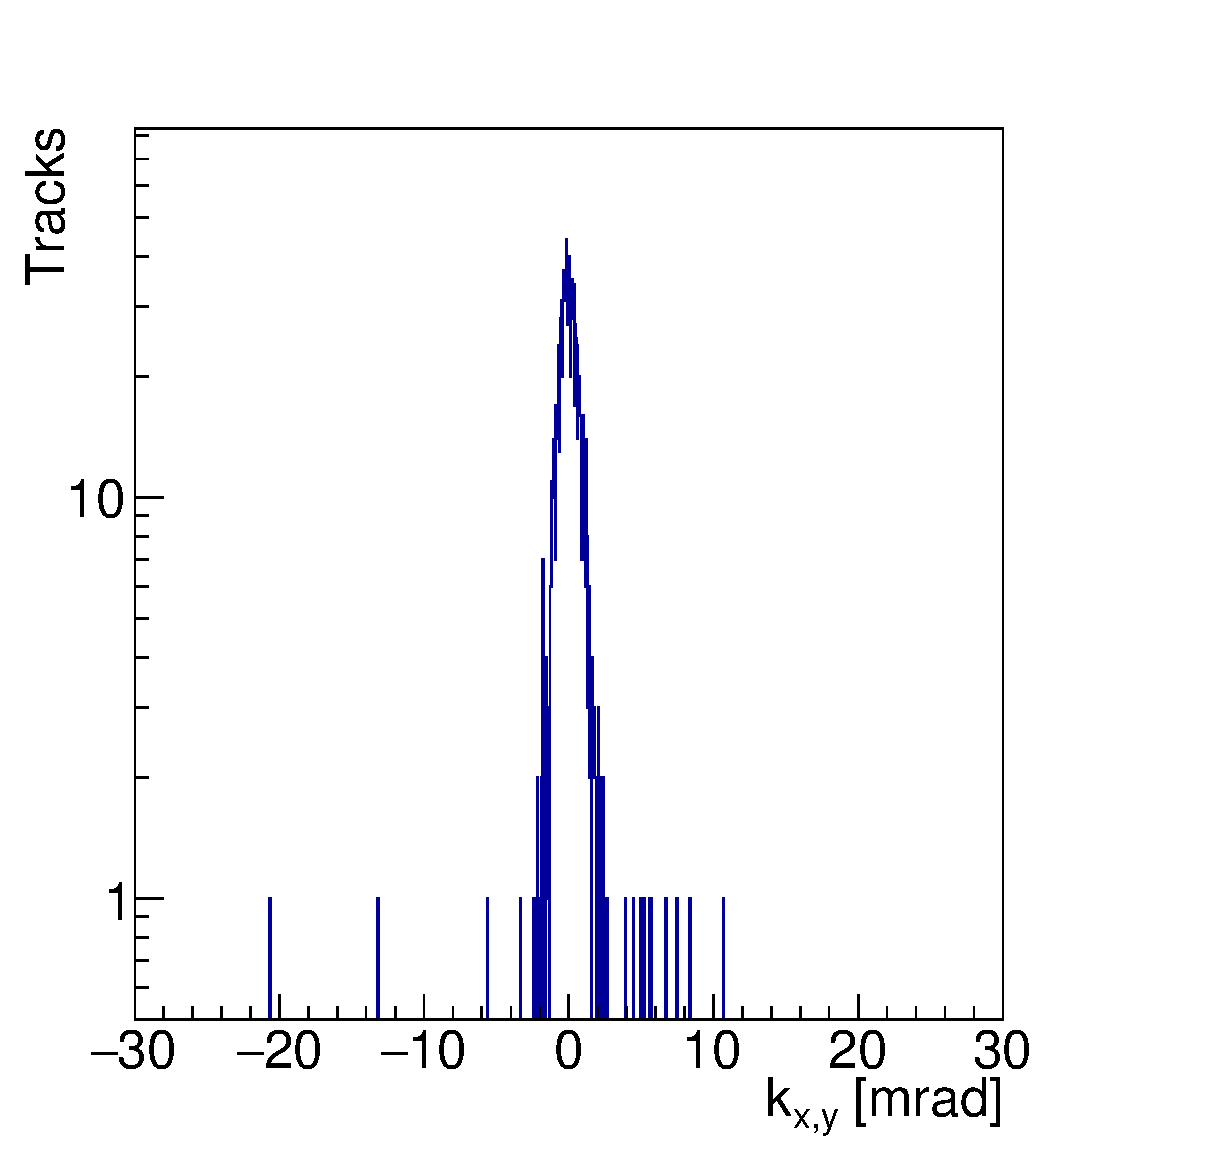
\includegraphics[width=0.45\textwidth]{figures/oneDistributionLogy.eps} \put(-165, 170){(A)}\hspace{0.02\textwidth}
  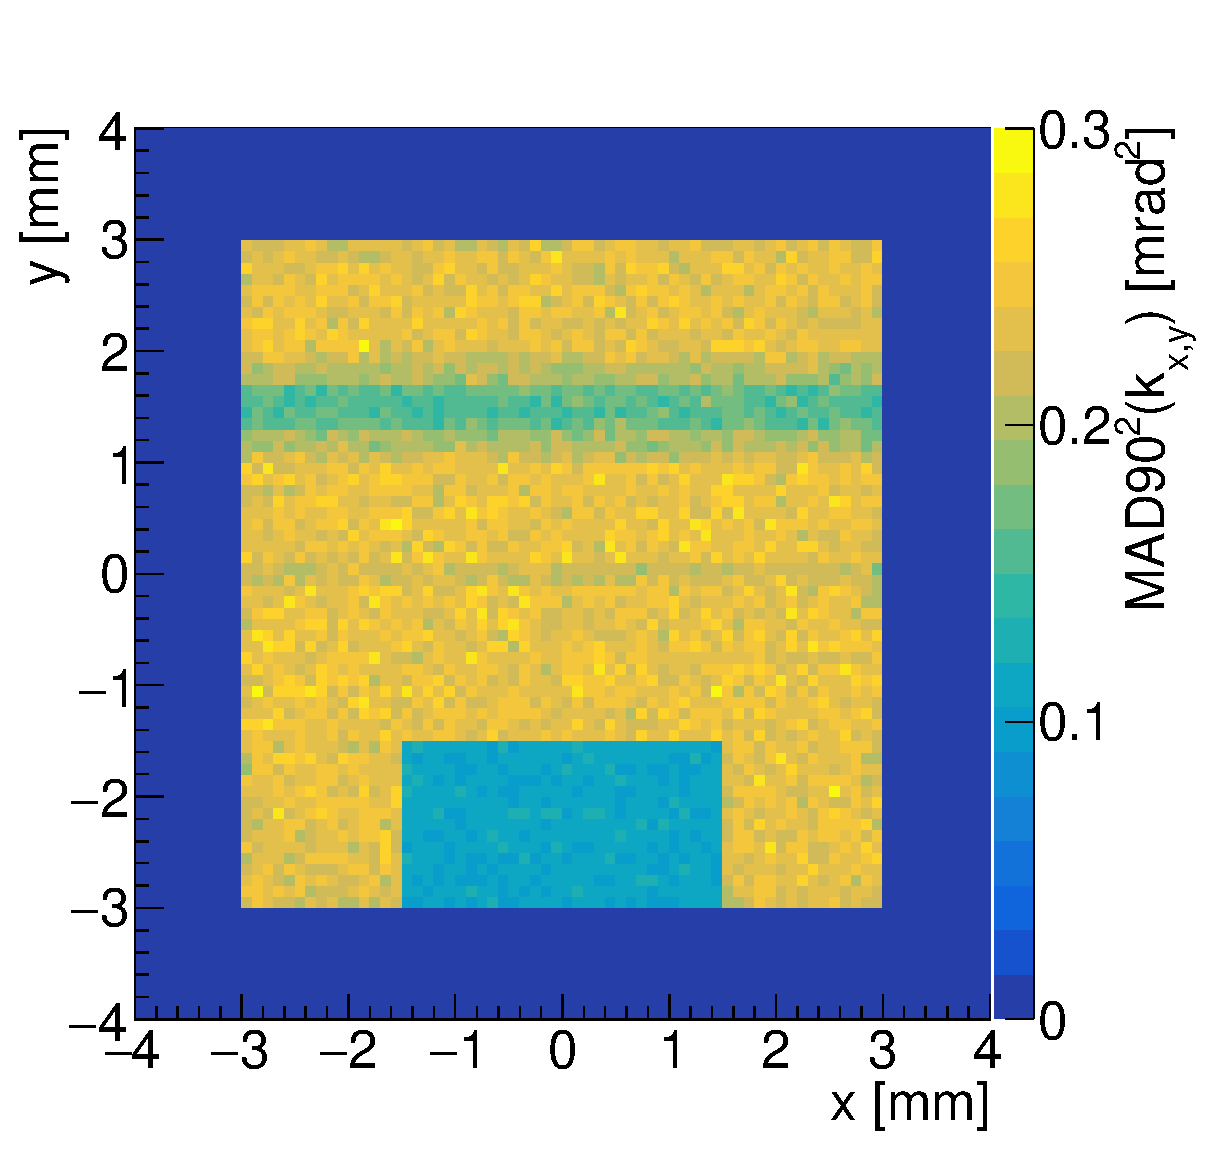
\includegraphics[width=0.45\textwidth]{figures/2Dxy.eps} \put(-165, 170){(B)}\\%
    \caption[angle distribution]{%
    (A) }
  \label{fig:angledistries}
\end{figure}

In the plane of the SUT, scattering angle distributions are created for cells of size $\SI{40}{\um} \times \SI{40}{\um}$. 
With a total number of XX simulated electron trajectories, the average number of tracks per image cell amounts to ..., the RMS of the number of tracks is ... .
The scattering angle distribution within one cell with X tracks, is shown in figure~\ref{fig:angledistries} (A).
From these distributions, the width in every cell is estimated. 
The statistics available for a given cell at a given cell size varies significantly, and therefore also the statistical uncertainty on the width of the scattering angle distribution. 
Additionally, due to a fluctuating number of outliers in a given cell, different estimators result in different estimates of the width as their sensitivity to outliers differ. 
Therefore, we construct various estimators of the width of the scattering angle distribution and compare their performance. 

%\setlength{\itemsep}{-10mm}
A priori, no absolute limit on the scattering angle is imposed in order not to bias the distribution before performing the estimation. 
The following estimators are compared:
\begin{itemize}\itemsep0pt
 \item RMS of a) the full data set ($\rmshundred$), b) the inner 90\% quantile ($\rmsninety$)
 \item Gaussian fit to c) the full data set ($\gausshundred$), d) the inner 95\% quantile ($\gaussninety$)
 \item Student t plus Gaussian fit to e) the full data set ($\studhundred$), f) the inner 95\% quantile ($\studninety$)
 \item Average absolute deviation of g) the full data set ($\aadhundred$), g) the inner 90\% quantile ($\aadninety$)
 
\end{itemize}

An example of the two dimensional distribution at a sample rotation angle of $\varphi = \SI{0}{\degree}$ is shown in figure~\ref{fig:angledistries} (B). 

%criteria:
%
%- robust (dependence on population)
%- accurate (similar to HL)
%- unbiased (no boundaries while filling)

Figure~\ref{fig:estis} shows the width distribution for the $\rmsninety$ estimator. 
Clearly distinguishable are the regions of air, and the various thicknesses of aluminium, c.f.\ figure~\ref{fig:setup}. 

\begin{figure}[t!]
  \centering
  %\includegraphics[width=0.49\textwidth]{img/run28_1GeV_01mm_gblsumkxandsumky_xyP_mean.eps}  
  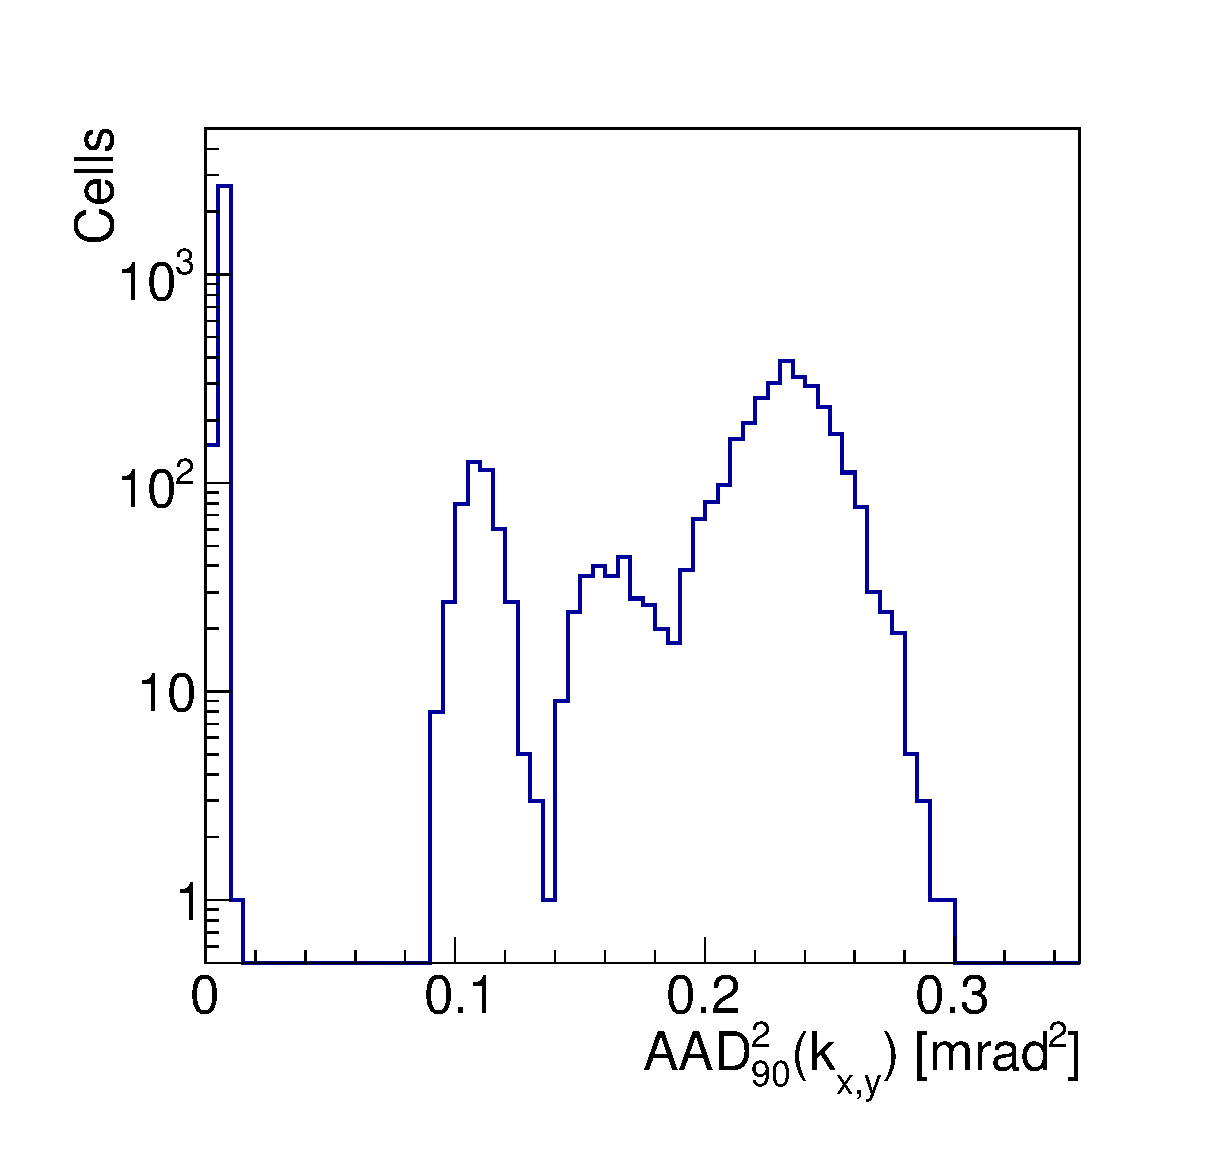
\includegraphics[width=0.45\textwidth]{figures/signalDistLogy.eps} \put(-165, 170){(A)}\hspace{0.02\textwidth}
  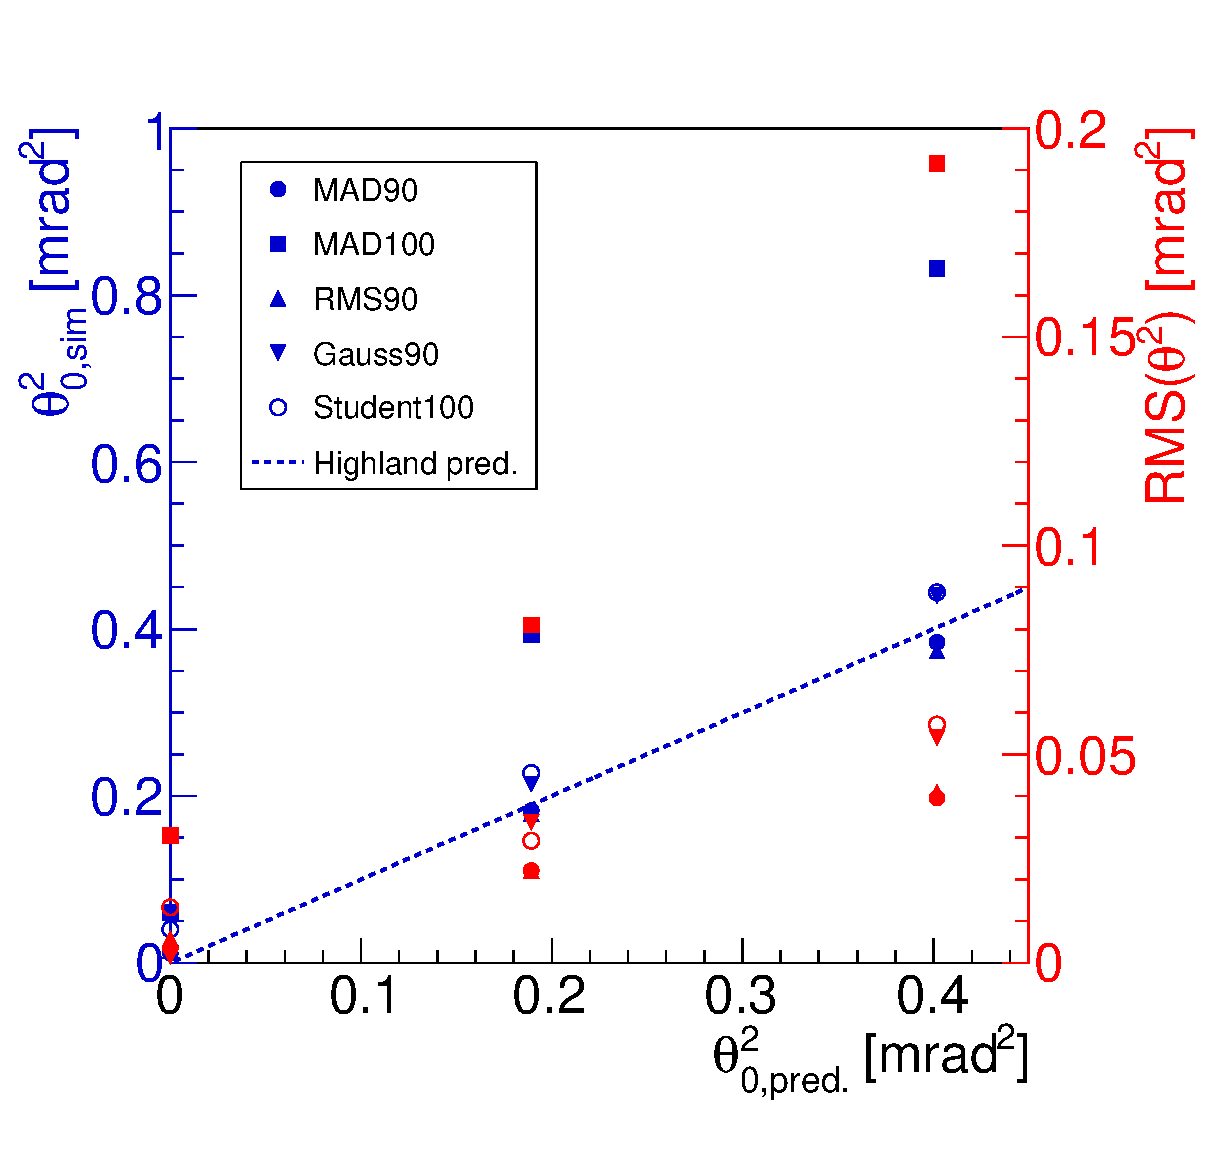
\includegraphics[width=0.45\textwidth]{figures/estimators1.eps} \put(-165, 170){(B)}\\%
    \caption[estimator distribution]{%
    (A) The distribution of the width for the $\rmsninety$ estimator is shown. The vertical line represents the Highland prediction.
    (B) The mean and RMS of various estimators are compared to the Highland prediction for various thicknesses. }
  \label{fig:estis}
\end{figure}

\section{Results}

at voxel size ... and fixed number of tracks.

\paragraph{Contrast}

The contrast to noise ratio (CNR) of the reconstructed image is evaluated for all estimators. 
As expected, the image CNR is best for the estimator with the smallest variance in the input values. 
Also, the image performance of the other estimators follows their 2D performance. 
In figure~\ref{fig:contrast}, the reconstructed image is shown for $\rmsninety$ (left) and $\rmshundred$ (right).

\begin{figure}[t!]
  \centering
  %\includegraphics[width=0.49\textwidth]{img/run28_1GeV_01mm_gblsumkxandsumky_xyP_mean.eps}  
  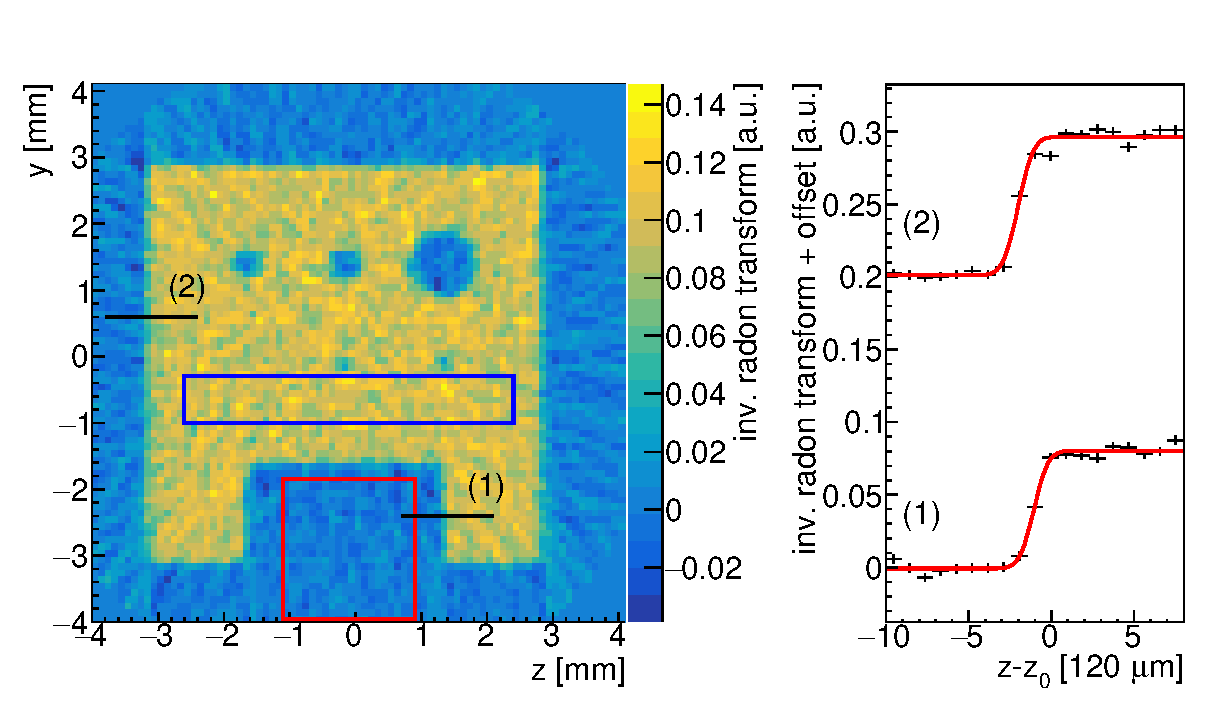
\includegraphics[width=0.48\textwidth]{figures/edgesMAD90.eps} \put(-115, 115){(A)}\hspace{0.02\textwidth}
  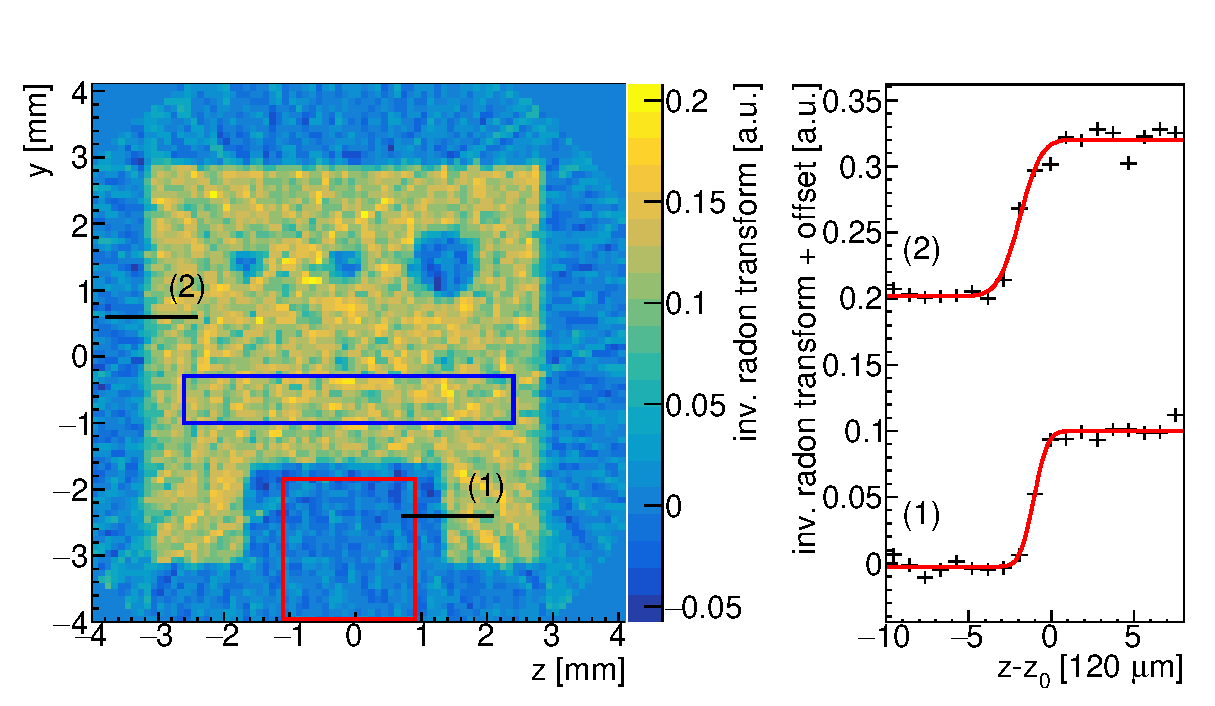
\includegraphics[width=0.48\textwidth]{figures/edgesRMS95.eps} \put(-115, 115){(B)}\\%
    \caption[contrast]{%
    (A) Contrast and reso for estimator h) (AAD$_{90}$).. %FIXME
    (B) Contrast and reso for estimator  a+b/2 (rms$_{95}$)}
  \label{fig:contrast}
\end{figure}

\paragraph{Resolution}

The edge resolution of the reconstructed image is evaluated for all estimators. 
As expected, the image edge resolution is best for the estimator with the smallest variance in the input values. 
Also, the image performance of the other estimators follows their 2D performance. 
In figure~\ref{fig:contrast}, the right-hand boxes show the edge resolution for $\rmsninety$ (left) and $\rmshundred$ (right).

\paragraph{Resolution vs contrast}

%- reso vs contrast for various bin sizes
Both the contrast and the edge resolution depend on the voxel size. 
With smaller voxel sizes the number of tracks per voxel decreases, increasing the image noise and hence decreasing contrast.
Within a certain range (... to ...), the decrased voxel size positively influences the image resolution. 

\begin{figure}[t!]
  \centering
  %\includegraphics[width=0.49\textwidth]{img/run28_1GeV_01mm_gblsumkxandsumky_xyP_mean.eps}  
  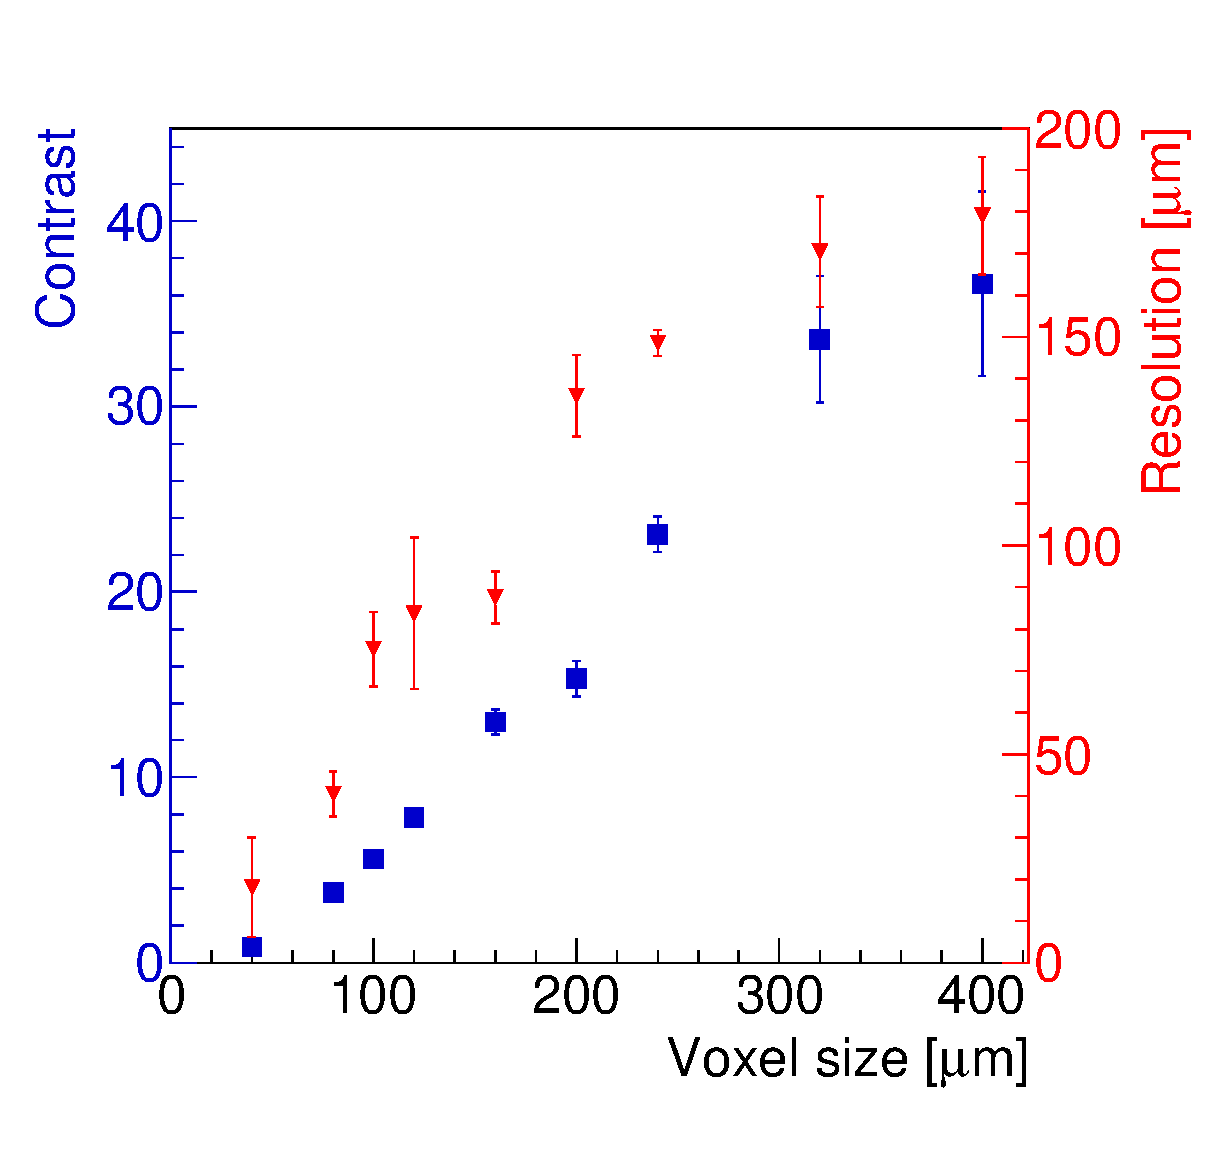
\includegraphics[width=0.70\textwidth]{figures/CRvsVS.eps}
    \caption[contrast]{%
    Reso vs contrast for various voxel sizes}
  \label{fig:resovscontrast}
\end{figure}


\section{Conclusion}

We reported on simulations regarding material budget measurements using beam telescopes and GeV electrons. 
The contrast of the image reconstructed from scattering angle distributions depends on the choice of the width estimator, especially at small statistics. 
The estimator with the smallest variance was found to be ... resulting in an image CNR of $\SI{6.0}{6}$  at a voxel size of ... . % FIXME
For the best performing estimator, the voxel size was varied affecting the image resolution and image contrast. 
We found the resolution and contrast to be empirically described by reso = constant*1/(voxel cube length)**3/2, contrast = constant*...




\bibliographystyle{unsrt}
\bibliography{bibtex/refs}

\end{document}
